\documentclass[a4paper,12pt]{article} % This defines the style of your paper

\usepackage[top = 2.5cm, bottom = 2.5cm, left = 2.5cm, right = 2.5cm]{geometry} 

% Unfortunately, LaTeX has a hard time interpreting German Umlaute. The following two lines and packages should help. If it doesn't work for you please let me know.
\usepackage[T1]{fontenc}
\usepackage[utf8]{inputenc}
\usepackage{pifont}
% \usepackage{ctex}
\usepackage{amsthm, amsmath, amssymb, mathrsfs,mathtools}
% ---------------------------------------------------------------------
% Program: listings-stata.tex
% Author:  github.com/mcaceresb
% Purpose: Stata language definition for LaTeX listings package
% Usage:   Add \input{listings-stata.tex} to your preamble

% Syntax from
% - https://github.com/isagalaev/highlight.js/blob/master/src/languages/stata.js
% - https://github.com/jpitblado/vim-stata/blob/master/syntax/stata.vim
% - http://fmwww.bc.edu/RePEc/bocode/s/synlightlist.ado

\RequirePackage{listings}
\RequirePackage{color}
\RequirePackage[svgnames]{xcolor}
\definecolor{spRed}{HTML}{BE646C}

% ---------------------------------------------------------------------
% Stata language definition

\lstdefinelanguage{stata}{
  sensitive=true,
  %
  % Macros, global and local
  alsoletter={\{\}0123456789},
  keywordsprefix=\$,
  morecomment=[n][keywordstyle9]{`}{'},
  morekeywords={},
  %
  % Comments
  morecomment=[f][\color{Green}\slshape][0]*,
  morecomment=[l]{//},
  morecomment=[s]{/*}{*/},
  %
  % Strings
  morecomment=[n][\color{Maroon}]{`"}{"'},
  morestring=[b]",
  %
  % Add-ons and system Commands
  morekeywords=[2]{
    if ,else ,in ,foreach ,for ,forv ,forva ,forval ,forvalu ,forvalue
    ,forvalues ,by ,bys ,bysort ,xi ,quietly ,qui ,capture ,about
    ,ac ,ac_7 ,acprplot ,acprplot_7 adjust ,ado ,adopath ,adoupdate
    ,alpha ,ameans ,an ,ano ,anov ,anova ,anova_estat ,anova_terms
    ,anovadef ,aorder ,ap ,app ,appe ,appen ,append ,arch ,arch_dr
    ,arch_estat ,arch_p ,archlm ,areg ,areg_p ,args ,arima ,arima_dr
    ,arima_estat ,arima_p ,as ,asmprobit ,asmprobit_estat ,asmprobit_lf
    ,asmprobit_mfx__dlg ,asmprobit_p ,ass ,asse ,asser ,assert ,avplot
    ,avplot_7 ,avplots ,avplots_7 bcskew0 ,bgodfrey ,binreg ,bip0_lf
    ,biplot ,bipp_lf ,bipr_lf ,bipr_p ,biprobit ,bitest ,bitesti
    ,bitowt ,blogit ,bmemsize ,boot ,bootsamp ,bootstrap ,bootstrap_8
    ,boxco_l ,boxco_p ,boxcox ,boxcox_6 ,boxcox_p ,bprobit ,br ,break
    ,brier ,bro ,brow ,brows ,browse ,brr ,brrstat ,bs ,bs_7 ,bsampl_w
    ,bsample ,bsample_7 ,bsqreg ,bstat ,bstat_7 ,bstat_8 ,bstrap
    ,bstrap_7 ,ca ,ca_estat ,ca_p ,cabiplot ,camat ,canon ,canon_8
    ,canon_8_p ,canon_estat ,canon_p ,cap ,caprojection ,capt ,captu
    ,captur ,capture ,cat ,cc ,cchart ,cchart_7 ,cci ,cd ,censobs_table
    ,centile ,cf ,char ,chdir ,checkdlgfiles ,checkestimationsample
    ,checkhlpfiles ,checksum ,chelp ,ci ,cii ,cl ,class ,classutil
    ,clear ,cli ,clis ,clist ,clo ,clog ,clog_lf ,clog_p ,clogi
    ,clogi_sw ,clogit ,clogit_lf ,clogit_p ,clogitp ,clogl_sw ,cloglog
    ,clonevar ,clslistarray ,cluster ,cluster_measures ,cluster_stop
    ,cluster_tree ,cluster_tree_8 ,clustermat ,cmdlog ,cnr ,cnre
    ,cnreg ,cnreg_p ,cnreg_sw ,cnsreg ,codebook ,collaps4 ,collapse
    ,colormult_nb ,colormult_nw ,compare ,compress ,conf ,confi
    ,confir ,confirm ,conren ,cons ,const ,constr ,constra ,constrai
    ,constrain ,constraint ,continue ,contract ,copy ,copyright
    ,copysource ,cor ,corc ,corr ,corr2data ,corr_anti ,corr_kmo
    ,corr_smc ,corre ,correl ,correla ,correlat ,correlate ,corrgram
    ,cou ,coun ,count ,cox ,cox_p ,cox_sw ,coxbase ,coxhaz ,coxvar
    ,cprplot ,cprplot_7 ,crc ,cret ,cretu ,cretur ,creturn ,cross ,cs
    ,cscript ,cscript_log ,csi ,ct ,ct_is ,ctset ,ctst_5 ,ctst_st
    ,cttost ,cumsp ,cumsp_7 ,cumul ,cusum ,cusum_7 ,cutil ,d ,datasig
    ,datasign ,datasigna ,datasignat ,datasignatu ,datasignatur
    ,datasignature ,datetof ,db ,dbeta ,de ,dec ,deco ,decod ,decode
    ,deff ,des ,desc ,descr ,descri ,describ ,describe ,destring
    ,dfbeta ,dfgls ,dfuller ,di ,di_g ,dir ,dirstats ,dis ,discard
    ,disp ,disp_res ,disp_s ,displ ,displa ,display ,distinct ,do
    ,doe ,doed ,doedi ,doedit ,dotplot ,dotplot_7 ,dprobit ,drawnorm
    ,drop ,ds ,ds_util ,dstdize ,duplicates ,durbina ,dwstat ,dydx ,e
    ,ed ,edi ,edit ,egen ,eivreg ,emdef ,en ,enc ,enco ,encod ,encode
    ,eq ,erase ,ereg ,ereg_lf ,ereg_p ,ereg_sw ,ereghet ,ereghet_glf
    ,ereghet_glf_sh ,ereghet_gp ,ereghet_ilf ,ereghet_ilf_sh ,ereghet_ip
    ,eret ,eretu ,eretur ,ereturn ,err ,erro ,error ,est ,est_cfexist
    ,est_cfname ,est_clickable ,est_expand ,est_hold ,est_table
    ,est_unhold ,est_unholdok ,estat ,estat_default ,estat_summ
    ,estat_vce_only ,esti ,estimates ,etodow ,etof ,etomdy ,ex ,exi
    ,exit ,expand ,expandcl ,fac ,fact ,facto ,factor ,factor_estat
    ,factor_p ,factor_pca_rotated ,factor_rotate ,factormat ,fcast
    ,fcast_compute ,fcast_graph ,fdades ,fdadesc ,fdadescr ,fdadescri
    ,fdadescrib ,fdadescribe ,fdasav ,fdasave ,fdause ,fh_st ,file
    ,open ,file ,read ,file ,close ,file ,filefilter ,fillin
    ,find_hlp_file ,findfile ,findit ,findit_7 ,fit ,fl ,fli ,flis
    ,flist ,for5_0 ,form ,forma ,format ,fpredict ,frac_154 ,frac_adj
    ,frac_chk ,frac_cox ,frac_ddp ,frac_dis ,frac_dv ,frac_in ,frac_mun
    ,frac_pp ,frac_pq ,frac_pv ,frac_wgt ,frac_xo ,fracgen ,fracplot
    ,fracplot_7 ,fracpoly ,fracpred ,fron_ex ,fron_hn ,fron_p ,fron_tn
    ,fron_tn2 ,frontier ,ftodate ,ftoe ,ftomdy ,ftowdate ,g ,gamhet_glf
    ,gamhet_gp ,gamhet_ilf ,gamhet_ip ,gamma ,gamma_d2 ,gamma_p
    ,gamma_sw ,gammahet ,gdi_hexagon ,gdi_spokes ,ge ,gen ,gene ,gener
    ,genera ,generat ,generate ,genrank ,genstd ,genvmean ,gettoken
    ,gl ,gladder ,gladder_7 ,glim_l01 ,glim_l02 glim_l03 ,glim_l04
    ,glim_l05 ,glim_l06 ,glim_l07 ,glim_l08 ,glim_l09 ,glim_l10 glim_l11
    ,glim_l12 ,glim_lf ,glim_mu ,glim_nw1 ,glim_nw2 ,glim_nw3 ,glim_p
    ,glim_v1 ,glim_v2 ,glim_v3 ,glim_v4 ,glim_v5 ,glim_v6 ,glim_v7 ,glm
    ,glm_6 glm_p ,glm_sw ,glmpred ,glo ,glob ,globa ,global ,glogit
    ,glogit_8 ,glogit_p ,gmeans ,gnbre_lf ,gnbreg ,gnbreg_5 ,gnbreg_p
    ,gomp_lf ,gompe_sw ,gomper_p ,gompertz ,gompertzhet ,gomphet_glf
    ,gomphet_glf_sh ,gomphet_gp ,gomphet_ilf ,gomphet_ilf_sh ,gomphet_ip
    ,gphdot ,gphpen ,gphprint ,gprefs ,gprobi_p ,gprobit ,gprobit_8
    ,gr ,gr7 ,gr_copy ,gr_current ,gr_db ,gr_describe ,gr_dir ,gr_draw
    ,gr_draw_replay ,gr_drop ,gr_edit ,gr_editviewopts ,gr_example
    ,gr_example2 gr_export ,gr_print ,gr_qscheme ,gr_query ,gr_read
    ,gr_rename ,gr_replay ,gr_save ,gr_set ,gr_setscheme ,gr_table
    ,gr_undo ,gr_use ,graph ,graph7 grebar ,greigen ,greigen_7
    ,greigen_8 ,grmeanby ,grmeanby_7 ,gs_fileinfo ,gs_filetype
    ,gs_graphinfo ,gs_stat ,gsort ,gwood ,h ,hadimvo ,hareg ,hausman
    ,haver ,he ,heck_d2 ,heckma_p ,heckman ,heckp_lf ,heckpr_p ,heckprob
    ,hel ,help ,hereg ,hetpr_lf ,hetpr_p ,hetprob ,hettest ,hexdump
    ,hilite ,hist ,hist_7 histogram ,hlogit ,hlu ,hmeans ,hotel
    ,hotelling ,hprobit ,hreg ,hsearch ,icd9 ,icd9_ff ,icd9p ,iis
    ,impute ,imtest ,inbase ,include ,inf ,infi ,infil ,infile ,infix
    ,inp ,inpu ,input ,ins ,insheet ,insp ,inspe ,inspec ,inspect ,integ
    ,inten ,intreg ,intreg_7 ,intreg_p ,intrg2_ll ,intrg_ll ,intrg_ll2
    ,ipolate ,iqreg ,ir ,irf ,irf_create ,irfm ,iri ,is_svy ,is_svysum
    ,isid ,istdize ,ivprob_1_lf ,ivprob_lf ,ivprobit ,ivprobit_p ,ivreg
    ,ivreg_footnote ,ivtob_1_lf ,ivtob_lf ,ivtobit ,ivtobit_p ,jackknife
    ,jacknife ,jknife ,jknife_6 ,jknife_8 ,jkstat ,joinby ,kalarma1
    ,kap ,kap_3 ,kapmeier ,kappa ,kapwgt ,kdensity ,kdensity_7 keep
    ,ksm ,ksmirnov ,ktau ,kwallis ,l ,la ,lab ,labe ,label ,labelbook
    ,ladder ,levels ,levelsof ,leverage ,lfit ,lfit_p ,li ,lincom ,line
    ,linktest ,lis ,list ,lloghet_glf ,lloghet_glf_sh ,lloghet_gp
    ,lloghet_ilf ,lloghet_ilf_sh ,lloghet_ip ,llogi_sw ,llogis_p
    ,llogist ,llogistic ,llogistichet ,lnorm_lf ,lnorm_sw ,lnorma_p
    ,lnormal ,lnormalhet ,lnormhet_glf ,lnormhet_glf_sh ,lnormhet_gp
    ,lnormhet_ilf ,lnormhet_ilf_sh ,lnormhet_ip ,lnskew0 ,loadingplot
    ,loc ,loca ,local ,log ,logi ,logis_lf ,logistic ,logistic_p
    ,logit ,logit_estat ,logit_p ,loglogs ,logrank ,loneway ,lookfor
    ,lookup ,lowess ,lowess_7 ,lpredict ,lrecomp ,lroc ,lroc_7 ,lrtest
    ,ls ,lsens ,lsens_7 ,lsens_x ,lstat ,ltable ,ltable_7 ,ltriang
    ,lv ,lvr2plot ,lvr2plot_7 ,m ,ma ,mac ,macr ,macro ,makecns ,man
    ,manova ,manova_estat ,manova_p ,manovatest ,mantel ,mark ,markin
    ,markout ,marksample ,mat ,mat_capp ,mat_order ,mat_put_rr ,mat_rapp
    ,mata ,mata_clear ,mata_describe ,mata_drop ,mata_matdescribe
    ,mata_matsave ,mata_matuse ,mata_memory ,mata_mlib ,mata_mosave
    ,mata_rename ,mata_which ,matalabel ,matcproc ,matlist ,matname
    ,matr ,matri ,matrix ,matrix_input__dlg ,matstrik ,mcc ,mcci ,md0_
    ,md1_ ,md1debug_ ,md2_ ,md2debug_ ,mds ,mds_estat ,mds_p ,mdsconfig
    ,mdslong ,mdsmat ,mdsshepard ,mdytoe ,mdytof ,me_derd ,mean ,means
    ,median ,memory ,memsize ,meqparse ,mer ,merg ,merge ,mfp ,mfx
    ,mhelp ,mhodds ,minbound ,mixed_ll ,mixed_ll_reparm ,mkassert
    ,mkdir ,mkmat ,mkspline ,ml ,ml_5 ml_adjs ,ml_bhhhs ,ml_c_d
    ,ml_check ,ml_clear ,ml_cnt ,ml_debug ,ml_defd ,ml_e0 ml_e0_bfgs
    ,ml_e0_cycle ,ml_e0_dfp ,ml_e0i ,ml_e1 ,ml_e1_bfgs ,ml_e1_bhhh
    ,ml_e1_cycle ,ml_e1_dfp ,ml_e2 ,ml_e2_cycle ,ml_ebfg0 ,ml_ebfr0
    ,ml_ebfr1 ml_ebh0q ,ml_ebhh0 ,ml_ebhr0 ,ml_ebr0i ,ml_ecr0i ,ml_edfp0
    ,ml_edfr0 ,ml_edfr1 ml_edr0i ,ml_eds ,ml_eer0i ,ml_egr0i ,ml_elf
    ,ml_elf_bfgs ,ml_elf_bhhh ,ml_elf_cycle ,ml_elf_dfp ,ml_elfi
    ,ml_elfs ,ml_enr0i ,ml_enrr0 ,ml_erdu0 ml_erdu0_bfgs ,ml_erdu0_bhhh
    ,ml_erdu0_bhhhq ,ml_erdu0_cycle ,ml_erdu0_dfp ,ml_erdu0_nrbfgs
    ,ml_exde ,ml_footnote ,ml_geqnr ,ml_grad0 ,ml_graph ,ml_hbhhh
    ,ml_hd0 ,ml_hold ,ml_init ,ml_inv ,ml_log ,ml_max ,ml_mlout
    ,ml_mlout_8 ,ml_model ,ml_nb0 ,ml_opt ,ml_p ,ml_plot ,ml_query
    ,ml_rdgrd ,ml_repor ,ml_s_e ,ml_score ,ml_searc ,ml_technique
    ,ml_unhold ,mleval ,mlf_ ,mlmatbysum ,mlmatsum ,mlog ,mlogi ,mlogit
    ,mlogit_footnote ,mlogit_p ,mlopts ,mlsum ,mlvecsum ,mnl0_ ,mor
    ,more ,mov ,move ,mprobit ,mprobit_lf ,mprobit_p ,mrdu0_ ,mrdu1_
    ,mvdecode ,mvencode ,mvreg ,mvreg_estat ,n ,nbreg ,nbreg_al
    ,nbreg_lf ,nbreg_p ,nbreg_sw ,nestreg ,net ,newey ,newey_7 ,newey_p
    ,news ,nl ,nl_7 ,nl_9 ,nl_9_p ,nl_p ,nl_p_7 nlcom ,nlcom_p ,nlexp2
    ,nlexp2_7 ,nlexp2a ,nlexp2a_7 ,nlexp3 ,nlexp3_7 ,nlgom3 nlgom3_7
    ,nlgom4 ,nlgom4_7 ,nlinit ,nllog3 ,nllog3_7 ,nllog4 ,nllog4_7
    ,nlog_rd ,nlogit ,nlogit_p ,nlogitgen ,nlogittree ,nlpred ,no
    ,nobreak ,noi ,nois ,noisi ,noisil ,noisily ,note ,notes ,notes_dlg
    ,nptrend ,numlabel ,numlist ,odbc ,old_ver ,olo ,olog ,ologi
    ,ologi_sw ,ologit ,ologit_p ,ologitp ,on ,one ,onew ,onewa ,oneway
    ,op_colnm ,op_comp ,op_diff ,op_inv ,op_str ,opr ,opro ,oprob
    ,oprob_sw ,oprobi ,oprobi_p ,oprobit ,oprobitp ,opts_exclusive
    ,order ,orthog ,orthpoly ,ou ,out ,outf ,outfi ,outfil ,outfile
    ,outs ,outsh ,outshe ,outshee ,outsheet ,ovtest ,pac ,pac_7 ,palette
    ,parse ,parse_dissim ,pause ,pca ,pca_8 pca_display ,pca_estat
    ,pca_p ,pca_rotate ,pcamat ,pchart ,pchart_7 ,pchi ,pchi_7 ,pcorr
    ,pctile ,pentium ,pergram ,pergram_7 ,permute ,permute_8 ,personal
    ,peto_st ,pkcollapse ,pkcross ,pkequiv ,pkexamine ,pkexamine_7
    ,pkshape ,pksumm ,pksumm_7 ,pl ,plo ,plot ,plugin ,pnorm ,pnorm_7
    ,poisgof ,poiss_lf ,poiss_sw ,poisso_p ,poisson ,poisson_estat
    ,post ,postclose ,postfile ,postutil ,pperron ,pr ,prais ,prais_e
    ,prais_e2 ,prais_p ,predict ,predictnl ,preserve ,print ,pro ,prob
    ,probi ,probit ,probit_estat ,probit_p ,proc_time ,procoverlay
    ,procrustes ,procrustes_estat ,procrustes_p ,profiler ,prog ,progr
    ,progra ,program ,prop ,proportion ,prtest ,prtesti ,pwcorr ,pwd
    ,q ,s ,qby ,qbys ,qchi ,qchi_7 ,qladder ,qladder_7 ,qnorm ,qnorm_7
    ,qqplot ,qqplot_7 ,qreg ,qreg_c ,qreg_p ,qreg_sw ,qu ,quadchk
    ,quantile ,quantile_7 ,que ,quer ,query ,range ,ranksum ,ratio
    ,rchart ,rchart_7 ,rcof ,recast ,reclink ,recode ,reg ,reg3
    ,reg3_p ,regdw ,regr ,regre ,regre_p2 ,regres ,regres_p ,regress
    ,regress_estat ,regriv_p ,remap ,ren ,rena ,renam ,rename ,renpfix
    ,repeat ,replace ,report ,reshape ,restore ,ret ,retu ,retur ,return
    ,rm ,rmdir ,robvar ,roccomp ,roccomp_7 ,roccomp_8 ,rocf_lf ,rocfit
    ,rocfit_8 ,rocgold ,rocplot ,rocplot_7 ,roctab ,roctab_7 ,rolling
    ,rologit ,rologit_p ,rot ,rota ,rotat ,rotate ,rotatemat ,rreg
    ,rreg_p ,ru ,run ,runtest ,rvfplot ,rvfplot_7 ,rvpplot ,rvpplot_7
    ,sa ,safesum ,sample ,sampsi ,sav ,save ,savedresults ,saveold ,sc
    ,sca ,scal ,scala ,scalar ,scatter ,scm_mine ,sco ,scob_lf ,scob_p
    ,scobi_sw ,scobit ,scor ,score ,scoreplot ,scoreplot_help ,scree
    ,screeplot ,screeplot_help ,sdtest ,sdtesti ,se ,search ,separate
    ,seperate ,serrbar ,serrbar_7 ,serset ,set ,set_defaults ,sfrancia
    ,sh ,she ,shel ,shell ,shewhart ,shewhart_7 ,signestimationsample
    ,signrank ,signtest ,simul ,simul_7 simulate ,simulate_8 ,sktest
    ,sleep ,slogit ,slogit_d2 ,slogit_p ,smooth ,snapspan ,so ,sor
    ,sort ,spearman ,spikeplot ,spikeplot_7 ,spikeplt ,spline_x ,split
    ,sqreg ,sqreg_p ,sret ,sretu ,sretur ,sreturn ,ssc ,st ,st_ct ,st_hc
    ,st_hcd ,st_hcd_sh ,st_is ,st_issys ,st_note ,st_promo ,st_set
    ,st_show ,st_smpl ,st_subid ,stack ,statsby ,statsby_8 ,stbase
    ,stci ,stci_7 ,stcox ,stcox_estat ,stcox_fr ,stcox_fr_ll ,stcox_p
    ,stcox_sw ,stcoxkm ,stcoxkm_7 ,stcstat ,stcurv ,stcurve ,stcurve_7
    ,stdes ,stem ,stepwise ,stereg ,stfill ,stgen ,stir ,stjoin ,stmc
    ,stmh ,stphplot ,stphplot_7 ,stphtest ,stphtest_7 ,stptime ,strate
    ,strate_7 ,streg ,streg_sw ,streset ,sts ,sts_7 ,stset ,stsplit
    ,stsum ,sttocc ,sttoct ,stvary ,stweib ,su ,suest ,suest_8 ,sum
    ,summ ,summa ,summar ,summari ,summariz ,summarize ,sunflower
    ,sureg ,survcurv ,survsum ,svar ,svar_p ,svmat ,svy ,svy_disp
    ,svy_dreg ,svy_est ,svy_est_7 ,svy_estat ,svy_get ,svy_gnbreg_p
    ,svy_head ,svy_header ,svy_heckman_p ,svy_heckprob_p ,svy_intreg_p
    ,svy_ivreg_p ,svy_logistic_p ,svy_logit_p ,svy_mlogit_p ,svy_nbreg_p
    ,svy_ologit_p ,svy_oprobit_p ,svy_poisson_p ,svy_probit_p
    ,svy_regress_p ,svy_sub ,svy_sub_7 ,svy_x ,svy_x_7 ,svy_x_p ,svydes
    ,svydes_8 ,svygen ,svygnbreg ,svyheckman ,svyheckprob ,svyintreg
    ,svyintreg_7 ,svyintrg ,svyivreg ,svylc ,svylog_p ,svylogit
    ,svymarkout ,svymarkout_8 ,svymean ,svymlog ,svymlogit ,svynbreg
    ,svyolog ,svyologit ,svyoprob ,svyoprobit ,svyopts ,svypois
    ,svypois_7 svypoisson ,svyprobit ,svyprobt ,svyprop ,svyprop_7
    ,svyratio ,svyreg ,svyreg_p ,svyregress ,svyset ,svyset_7 ,svyset_8
    ,svytab ,svytab_7 ,svytest ,svytotal ,sw ,sw_8 ,swcnreg ,swcox
    ,swereg ,swilk ,swlogis ,swlogit ,swologit ,swoprbt ,swpois
    ,swprobit ,swqreg ,swtobit ,swweib ,symmetry ,symmi ,symplot
    ,symplot_7 syntax ,sysdescribe ,sysdir ,sysuse ,szroeter ,ta ,tab
    ,tab1 ,tab2 ,tab_or ,tabd ,tabdi ,tabdis ,tabdisp ,tabi ,table
    ,tabodds ,tabodds_7 ,tabstat ,tabu ,tabul ,tabula ,tabulat ,tabulate
    ,te ,tempfile ,tempname ,tempvar ,tes ,test ,testnl ,testparm
    ,teststd ,tetrachoric ,time_it ,timer ,tis ,tob ,tobi ,tobit
    ,tobit_p ,tobit_sw ,token ,tokeni ,tokeniz ,tokenize ,tostring
    ,total ,translate ,translator ,transmap ,treat_ll ,treatr_p
    ,treatreg ,trim ,trnb_cons ,trnb_mean ,trpoiss_d2 ,trunc_ll
    ,truncr_p ,truncreg ,tsappend ,tset ,tsfill ,tsline ,tsline_ex
    ,tsreport ,tsrevar ,tsrline ,tsset ,tssmooth ,tsunab ,ttest
    ,ttesti ,tut_chk ,tut_wait ,tutorial ,tw ,tware_st ,two ,twoway
    ,twoway__fpfit_serset ,twoway__function_gen ,twoway__histogram_gen
    ,twoway__ipoint_serset ,twoway__ipoints_serset ,twoway__kdensity_gen
    ,twoway__lfit_serset ,twoway__normgen_gen ,twoway__pci_serset
    ,twoway__qfit_serset ,twoway__scatteri_serset ,twoway__sunflower_gen
    ,twoway_ksm_serset ,ty ,typ ,type ,typeof ,u ,unab ,unabbrev
    ,unabcmd ,update ,us ,use ,uselabel ,var ,var_mkcompanion
    ,var_p ,varbasic ,varfcast ,vargranger ,varirf ,varirf_add
    ,varirf_cgraph ,varirf_create ,varirf_ctable ,varirf_describe
    ,varirf_dir ,varirf_drop ,varirf_erase ,varirf_graph ,varirf_ograph
    ,varirf_rename ,varirf_set ,varirf_table ,varlist ,varlmar
    ,varnorm ,varsoc ,varstable ,varstable_w ,varstable_w2 ,varwle
    ,vce ,vec ,vec_fevd ,vec_mkphi ,vec_p ,vec_p_w ,vecirf_create
    ,veclmar ,veclmar_w ,vecnorm ,vecnorm_w ,vecrank ,vecstable
    ,verinst ,vers ,versi ,versio ,version ,view ,viewsource ,vif
    ,vwls ,wdatetof ,webdescribe ,webseek ,webuse ,weib1_lf ,weib2_lf
    ,weib_lf ,weib_lf0 weibhet_glf ,weibhet_glf_sh ,weibhet_glfa
    ,weibhet_glfa_sh ,weibhet_gp ,weibhet_ilf ,weibhet_ilf_sh
    ,weibhet_ilfa ,weibhet_ilfa_sh ,weibhet_ip ,weibu_sw ,weibul_p
    ,weibull ,weibull_c ,weibull_s ,weibullhet ,wh ,whelp ,whi ,which
    ,whil ,while ,wilc_st ,wilcoxon ,win ,wind ,windo ,window ,winexec
    ,wntestb ,wntestb_7 ,wntestq ,xchart ,xchart_7 ,xcorr ,xcorr_7 ,xi
    ,xi_6 ,xmlsav ,xmlsave ,xmluse ,xpose ,xsh ,xshe ,xshel ,xshell
    ,xt_iis ,xt_tis ,xtab_p ,xtabond ,xtbin_p ,xtclog ,xtcloglog
    ,xtcloglog_8 ,xtcloglog_d2 ,xtcloglog_pa_p ,xtcloglog_re_p ,xtcnt_p
    ,xtcorr ,xtdata ,xtdes ,xtfront_p ,xtfrontier ,xtgee ,xtgee_elink
    ,xtgee_estat ,xtgee_makeivar ,xtgee_p ,xtgee_plink ,xtgls ,xtgls_p
    ,xthaus ,xthausman ,xtht_p ,xthtaylor ,xtile ,xtint_p ,xtintreg
    ,xtintreg_8 ,xtintreg_d2 xtintreg_p ,xtivp_1 ,xtivp_2 ,xtivreg
    ,xtline ,xtline_ex ,xtlogit ,xtlogit_8 xtlogit_d2 ,xtlogit_fe_p
    ,xtlogit_pa_p ,xtlogit_re_p ,xtmixed ,xtmixed_estat ,xtmixed_p
    ,xtnb_fe ,xtnb_lf ,xtnbreg ,xtnbreg_pa_p ,xtnbreg_refe_p ,xtpcse
    ,xtpcse_p ,xtpois ,xtpoisson ,xtpoisson_d2 ,xtpoisson_pa_p
    ,xtpoisson_refe_p ,xtpred ,xtprobit ,xtprobit_8 ,xtprobit_d2
    ,xtprobit_re_p ,xtps_fe ,xtps_lf ,xtps_ren ,xtps_ren_8 ,xtrar_p
    ,xtrc ,xtrc_p ,xtrchh ,xtrefe_p ,xtreg ,xtreg_be ,xtreg_fe
    ,xtreg_ml ,xtreg_pa_p ,xtreg_re ,xtregar ,xtrere_p ,xtset
    ,xtsf_ll ,xtsf_llti ,xtsum ,xttab ,xttest0 ,xttobit ,xttobit_8
    ,xttobit_p ,xttrans ,yx ,yxview__barlike_draw ,yxview_area_draw
    ,yxview_bar_draw ,yxview_dot_draw ,yxview_dropline_draw
    ,yxview_function_draw ,yxview_iarrow_draw ,yxview_ilabels_draw
    ,yxview_normal_draw ,yxview_pcarrow_draw ,yxview_pcbarrow_draw
    ,yxview_pccapsym_draw ,yxview_pcscatter_draw ,yxview_pcspike_draw
    ,yxview_rarea_draw ,yxview_rbar_draw ,yxview_rbarm_draw
    ,yxview_rcap_draw ,yxview_rcapsym_draw ,yxview_rconnected_draw
    ,yxview_rline_draw ,yxview_rscatter_draw ,yxview_rspike_draw
    ,yxview_spike_draw ,yxview_sunflower_draw ,zap_s ,zinb ,zinb_llf
    ,zinb_plf ,zip ,zip_llf ,zip_p ,zip_plf ,zt_ct_5 ,zt_hc_5 ,zt_hcd_5
    ,zt_is_5 ,zt_iss_5 ,zt_sho_5 zt_smp_5 ,ztbase_5 ,ztcox_5 ,ztdes_5
    ,ztereg_5 ,ztfill_5 ,ztgen_5 ,ztir_5 ztjoin_5 ,ztnb ,ztnb_p ,ztp
    ,ztp_p ,zts_5 ,ztset_5 ,ztspli_5 ,ztsum_5 ,zttoct_5 ztvary_5
    ,ztweib_5
  },
  %
  % Built-in functions
  morekeywords=[3]{
    Cdhms ,Chms ,Clock ,Cmdyhms ,Cofc ,Cofd ,F ,Fden ,Ftail ,I ,J
    ,_caller ,abbrev ,abs ,acos ,acosh ,asin ,asinh ,atan ,atan2
    ,atanh ,autocode ,betaden ,binomial ,binomialp ,binomialtail
    ,binormal ,bofd ,byteorder ,c ,ceil ,char ,chi2 ,chi2den ,chi2tail
    ,cholesky ,chop ,clip ,clock ,cloglog ,cofC ,cofd ,colnumb ,colsof
    ,comb ,cond ,corr ,cos ,cosh ,d ,daily ,date ,day ,det ,dgammapda
    ,dgammapdada ,dgammapdadx ,dgammapdx ,dgammapdxdx ,dhms ,diag
    ,diag0cnt ,digamma ,dofC ,dofb ,dofc ,dofh ,dofm ,dofq ,dofw ,dofy
    ,dow ,doy ,dunnettprob ,e ,el ,epsdouble ,epsfloat ,exp ,fileexists
    ,fileread ,filereaderror ,filewrite ,float ,floor ,fmtwidth
    ,gammaden ,gammap ,gammaptail ,get ,group ,h ,hadamard ,halfyear
    ,halfyearly ,has_eprop ,hh ,hhC ,hms ,hofd ,hours ,hypergeometric
    ,hypergeometricp ,ibeta ,ibetatail ,index ,indexnot ,inlist
    ,inrange ,int ,inv ,invF ,invFtail ,invbinomial ,invbinomialtail
    ,invchi2 ,invchi2tail ,invcloglog ,invdunnettprob ,invgammap
    ,invgammaptail ,invibeta ,invibetatail ,invlogit ,invnFtail
    ,invnbinomial ,invnbinomialtail ,invnchi2 ,invnchi2tail ,invnibeta
    ,invnorm ,invnormal ,invnttail ,invpoisson ,invpoissontail ,invsym
    ,invt ,invttail ,invtukeyprob ,irecode ,issym ,issymmetric ,itrim
    ,length ,ln ,lnfact ,lnfactorial ,lngamma ,lnnormal ,lnnormalden
    ,log ,log10 ,logit ,lower ,ltrim ,m ,match ,matmissing ,matrix
    ,matuniform ,max ,maxbyte ,maxdouble ,maxfloat ,maxint ,maxlong ,mdy
    ,mdyhms ,mi ,mi ,min ,minbyte ,mindouble ,minfloat ,minint ,minlong
    ,minutes ,missing ,mm ,mmC ,mod ,mofd ,month ,monthly ,mreldif
    ,msofhours ,msofminutes ,msofseconds ,nF ,nFden ,nFtail ,nbetaden
    ,nbinomial ,nbinomialp ,nbinomialtail ,nchi2 ,nchi2den ,nchi2tail
    ,nibeta ,norm ,normal ,normalden ,normd ,npnF ,npnchi2 ,npnt ,nt
    ,ntden ,nttail ,nullmat ,plural ,poisson ,poissonp ,poissontail
    ,proper ,q ,qofd ,quarter ,quarterly ,r ,rbeta ,rbinomial ,rchi2
    real ,recode ,regexm ,regexr ,regexs ,reldif ,replay ,return
    ,reverse ,rgamma ,rhypergeometric ,rnbinomial ,rnormal ,round
    ,rownumb ,rowsof ,rpoisson ,rt ,rtrim ,runiform ,s ,scalar ,seconds
    ,sign ,sin ,sinh ,smallestdouble ,soundex ,soundex_nara ,sqrt ,ss
    ,ssC ,strcat ,strdup ,string ,strlen ,strlower ,strltrim ,strmatch
    ,strofreal ,strpos ,strproper ,strreverse ,strrtrim ,strtoname
    ,strtrim ,strupper ,subinstr ,subinword ,substr ,sum ,sweep ,syminv
    ,t ,tC ,tan ,tanh ,tc ,td ,tden ,th ,tin ,tm ,tq ,trace ,trigamma
    ,trim ,trunc ,ttail ,tukeyprob ,tw ,twithin ,uniform ,upper ,vec
    ,vecdiag ,w ,week ,weekly ,wofd ,word ,wordcount ,year ,yearly
    ,yh ,ym ,yofd ,yq ,yw
  },
  %
  % Numbers
  morekeywords=[4]{
    0 ,1 ,2 ,3 ,4 ,5 ,6 ,7 ,8 ,9
  },
}

% ---------------------------------------------------------------------
% Stata editor style

\providecommand{\textcolordummy}[2]{#2}
\lstalias{Stata}{stata}
\lstdefinestyle{stata-editor}{
    language=stata,
    %
    % Global variables
    keywordstyle={\bfseries\color{spRed}},
    %
    % Add-ons system commands
    keywordstyle=[2]{\bfseries\color{NavyBlue}},
    %
    % Built-in functions
    keywordstyle=[3]{\color{blue}},
    %
    % Numbers
    keywordstyle=[4]{\color{blue}},
    %
    % User macros (variables)
    keywordstyle = [9]{\bfseries\color{LightSteelBlue}\let\textcolor\textcolordummy},
    %
    % Strings and comments
    stringstyle  = \color{Maroon},
    commentstyle = \color{Green}\slshape,
}

% ---------------------------------------------------------------------
% Suggested settings

% \lstset{
%   basicstyle        = \setmonofont{DejaVu Sans Mono}\footnotesize\ttfamily,
%   tabsize           = 4,      % Tab size
%   showstringspaces  = false,  % Don't underline spaces in strings
%   showspaces        = false,  % Don't underline spaces
%   breaklines        = true,   % Automatic line breaking
%   breakatwhitespace = true,   % Breaks only at white space.
%   lineskip          = 1.5pt,  % Sparing between lines of code
%   commentstyle      = \color{black!50}\itshape \let\textcolor\textcolordummy,
% }

% Defining a new theorem style without italics
\newtheoremstyle{nonitalic}% name
  {\topsep}% Space above
  {\topsep}% Space below
  {\upshape}% Body font
  {}% Indent amount
  {\bfseries}% Theorem head font
  {.}% Punctuation after theorem head
  {.5em}% Space after theorem head
  {}% Theorem head spec (can be left empty, meaning ‘normal`)
  
\theoremstyle{nonitalic}
% Define new 'solution' environment
\newtheorem{innercustomsol}{Solution}
\newenvironment{solution}[1]
  {\renewcommand\theinnercustomsol{#1}\innercustomsol}
  {\endinnercustomsol}

% Custom counter for the solutions
\newcounter{solutionctr}
\renewcommand{\thesolutionctr}{(\alph{solutionctr})}

% Environment for auto-numbering with custom format
\newenvironment{autosolution}
  {\stepcounter{solutionctr}\begin{solution}{\thesolutionctr}}
  {\end{solution}}


\newtheorem{problem}{Problem}
\usepackage{color}

% The following two packages - multirow and booktabs - are needed to create nice looking tables.
\usepackage{multirow} % Multirow is for tables with multiple rows within one cell.
\usepackage{booktabs} % For even nicer tables.

% As we usually want to include some plots (.pdf files) we need a package for that.
\usepackage{graphicx} 
\usepackage{subfigure}


% The default setting of LaTeX is to indent new paragraphs. This is useful for articles. But not really nice for homework problem sets. The following command sets the indent to 0.
\usepackage{setspace}
\setlength{\parindent}{0in}
\usepackage{longtable}

% Package to place figures where you want them.
\usepackage{float}

% The fancyhdr package let's us create nice headers.
\usepackage{fancyhdr}

\usepackage{fancyvrb}

%Code environment 
\usepackage{listings} % Required for insertion of code
\usepackage{xcolor} % Required for custom colors

% Define colors for code listing
\definecolor{codegreen}{rgb}{0,0.6,0}
\definecolor{codegray}{rgb}{0.5,0.5,0.5}
\definecolor{codepurple}{rgb}{0.58,0,0.82}
\definecolor{backcolour}{rgb}{0.95,0.95,0.92}

% Code listing style named "mystyle"
\lstdefinestyle{mystyle}{
    backgroundcolor=\color{backcolour},   
    commentstyle=\color{codegreen},
    keywordstyle=\color{magenta},
    numberstyle=\tiny\color{codegray},
    stringstyle=\color{codepurple},
    basicstyle=\ttfamily\footnotesize, % Change to serif font
    breakatwhitespace=false,         
    breaklines=true,                 
    captionpos=b,                    
    keepspaces=true,                 
    numbers=left,                    
    numbersep=5pt,                  
    showspaces=false,                
    showstringspaces=false,
    showtabs=false,                  
    tabsize=2
}

\lstset{style=mystyle}

%%%%%%%%%%%%%%%%%%%%%%%%%%%%%%%%%%%%%%%%%%%%%%%%
% 3. Header (and Footer)
%%%%%%%%%%%%%%%%%%%%%%%%%%%%%%%%%%%%%%%%%%%%%%%%

% To make our document nice we want a header and number the pages in the footer.

\pagestyle{fancy} % With this command we can customize the header style.

\fancyhf{} % This makes sure we do not have other information in our header or footer.

\lhead{\footnotesize EI035 Econometrics II}% \lhead puts text in the top left corner. \footnotesize sets our font to a smaller size.

%\rhead works just like \lhead (you can also use \chead)
\rhead{\footnotesize Jingle Fu} %<---- Fill in your lastnames.

% Similar commands work for the footer (\lfoot, \cfoot and \rfoot).
% We want to put our page number in the center.
\cfoot{\footnotesize \thepage}
\IfFileExists{upquote.sty}{\usepackage{upquote}}{}
\begin{document}


\thispagestyle{empty} % This command disables the header on the first page. 

\begin{tabular}{p{15.5cm}} % This is a simple tabular environment to align your text nicely 
{\large \bf EI035 Econometrics II} \\
The Graduate Institute, Spring 2025, Marko Mlikota\\
\hline % \hline produces horizontal lines.
\\
\end{tabular} % Our tabular environment ends here.

\vspace*{0.3cm} % Now we want to add some vertical space in between the line and our title.

\begin{center} % Everything within the center environment is centered.
	{\Large \bf PS3 Solutions} % <---- Don't forget to put in the right number
	\vspace{2mm}
	
        % YOUR NAMES GO HERE
	{\bf Jingle Fu} % <---- Fill in your names here!
		
\end{center}  

\vspace{0.4cm}
\setstretch{1.2}

\begin{autosolution}
    \

    \begin{itemize}
        \item \textbf{Unit (Firm) Fixed Effects:}
        Each firm $i$ has intercept $\alpha_i$. When the number of firms $N$ is large but the time period $T$ is fixed,
        as $N$ increases, the number of these nuisance parameters increases too. The IPP refers to potential bias in the estimation of the structural parameters
        when the number of incidental parameters increases with the sample size.
        Such problem can lead to inconsistency in the estimation of the common parameters,
        because the estimation error in $\alpha_i$ doesn't vanish as $N \to \infty$.
        \item \textbf{Time Fixed Effects:}
        In contrast, time fixed effects add only $T$ dummies, the number of parameters associated with time dummies is fixed. 
        If we perform the within transformation as above, the time dummies remain in the model in the form
        \[\mathbf{1}\{t=\tau\} - \overline{d}_{it} \]
        and if we use first-differences, for any firm $i$, we have:
        \[\Delta  f_t = f_t - f_{t-1} \]
        Thus, the time fixed effects enter the differenced equation as differences, preserving their role in controlling for period-specific shocks.
        Hence, their estimation does not create an incidental parameters problem.
    \end{itemize}
    In short, while unit fixed effects can cause IPP when $T$ is relative small to $N$, 
    the addition of time fixed effects does not because the number of time dummies remains fixed and is asymptotically negligible.
    
% Table created by stargazer v.5.2.3 by Marek Hlavac, Social Policy Institute. E-mail: marek.hlavac at gmail.com
% Date and time: 周五, 11月 08, 2024 - 10:35:42
\begin{table}[!htbp] \centering 
  \caption{Regression with age^2} 
  \label{} 
\begin{tabular}{@{\extracolsep{5pt}}lc} 
\\[-1.8ex]\hline 
\hline \\[-1.8ex] 
 & \multicolumn{1}{c}{\textit{Dependent variable:}} \\ 
\cline{2-2} 
\\[-1.8ex] & log(ahe) \\ 
\hline \\[-1.8ex] 
 age & 0.081$^{*}$ \\ 
  & (0.043) \\ 
  & \\ 
 age2 & $-$0.001 \\ 
  & (0.001) \\ 
  & \\ 
 female & $-$0.186$^{***}$ \\ 
  & (0.011) \\ 
  & \\ 
 bachelor & 0.428$^{***}$ \\ 
  & (0.011) \\ 
  & \\ 
 Constant & 1.085$^{*}$ \\ 
  & (0.638) \\ 
  & \\ 
\hline \\[-1.8ex] 
Observations & 7,711 \\ 
R$^{2}$ & 0.201 \\ 
Adjusted R$^{2}$ & 0.200 \\ 
Residual Std. Error & 0.469 (df = 7706) \\ 
F Statistic & 484.078$^{***}$ (df = 4; 7706) \\ 
\hline 
\hline \\[-1.8ex] 
\textit{Note:}  & \multicolumn{1}{r}{$^{*}$p$<$0.1; $^{**}$p$<$0.05; $^{***}$p$<$0.01} \\ 
\end{tabular} 
\end{table} 

\begin{lstlisting}[language=stata]
use GMdata.dta, clear
xtset index yr
xtreg ldsal lemp ldnpt ldrst i.yr, fe robust
\end{lstlisting}
\end{autosolution}

\begin{autosolution}
    \


    For consecutive time periods $t$ and $t-1$, we take the difference and have:
    \[
    \Delta ldsal_{it} = \beta_1 \Delta lemp_{it} + \beta_2 \Delta ldnpt_{it} + \beta_3 \Delta ldrst_{it} + (f_t - f_{t-1}) + \Delta u_{it}
    \]
    Since $\alpha_i$ does not vary over time, it drops out in the differencing.
    For the dummies, we have:
    \begin{gather*}
        \mathbf{1}\{t=\tau\} - \mathbf{1}\{t-1=\tau\}=\begin{cases}
            +1 &\text{if } t=\tau,\\
            -1 &\text{if } t-1=\tau,\\
            0 &\text{otherwise.}
        \end{cases}
    \end{gather*}
    

    The time effects appear as differences $f_t - f_{t-1}$.
    Thus, in the first-differenced equation the levels of the year dummies disappear, but their differences remain. 
\end{autosolution}


\begin{autosolution}
    \

    Adding a time-invariant dummy variable to the regression $d357_i$, we get:
    \begin{gather*}
        ldsal_{it} = \alpha_i + \beta_1 lemp_{it} + \beta_2 ldnpt_{it} + \beta_3 ldrst_{it} + \delta d357_i + \sum_{\tau =1}^{T} f_t\mathbf{1}\{t=\tau\} + u_{it}
    \end{gather*}
    We take the first-differences of the equation:
    \[\Delta \delta d357_i = 0.\]
    Thus, in the first-difference model, the term $\delta d357_i$ drops out, and the time dummies are differenced out.
    The IPP arises from having many firm-specific parameters with a limited number of observations.
    So,including a time-invariant dummy does not worsen the IPP since it adds only one parameter that is either absorbed (or eliminated in first differences).

    If we consider Time-Varying Effects of the industry dummy $\delta_t d357_{it}$:
    taking the first-difference, we have:
    \[\Delta(\delta_t d357_{it}) = \delta_t d357_{it} - \delta_{t-1} d357_{i,t-1} = \delta_t - \delta_{t-1}\]
    as $\delta d357_{it} =1$ for all $t$ if the firm is in the computer industry.
    For firms not in industry 357, the term remains zero. Thus, in the first-difference equation, 
    the industry effect appears as the difference $\delta_t - \delta_{t-1}$, which is time-varying.

    Although allowing the industry effect to vary over time introduces several parameters,
    the number of these parameters is tied to the fixed. 
    And the key issue with IPP is the growth of parameters with $N$, which does not occur here.
\end{autosolution}

\begin{autosolution}
    \

    As we define $\ddot{y}_{it}= y_{it} - \overline{y}_{it}$ and $\ddot{X}_{it} - \overline{X}_{it}$, we have:
    \[
    \hat{\beta}_{FE-W} = \Bigl( \sum_{i,t} \ddot{X}_{it}^{\prime} \ddot{X}_{it} \Bigr) \sum_{i,t} \ddot{X}_{it} \ddot{y}_{it}
    \]
    \[
    \hat{\beta}_{RE} = \Bigl( X^{\prime} \Omega^{-1} X \Bigr)^{-1} X^{\prime} \Omega^{-1} y
    \]
    \begin{table}[htbp]\centering
\def\sym#1{\ifmmode^{#1}\else\(^{#1}\)\fi}
\caption{Fixed Effects Model}
\begin{tabular}{l*{1}{c}}
\toprule
                    &\multicolumn{1}{c}{(1)}\\
                    &\multicolumn{1}{c}{log of deflated sales}\\
                    &        b/se         \\
\midrule
log of employment   &       0.650\sym{***}\\
                    &     (0.031)         \\
log of deflated capital&       0.186\sym{***}\\
                    &     (0.025)         \\
log of deflated R\&D &       0.098\sym{***}\\
                    &     (0.019)         \\
year == 73, 78, 83, 88=73&       0.000         \\
                    &         (.)         \\
year == 73, 78, 83, 88=78&       0.058\sym{***}\\
                    &     (0.016)         \\
year == 73, 78, 83, 88=83&      -0.012         \\
                    &     (0.020)         \\
year == 73, 78, 83, 88=88&       0.251\sym{***}\\
                    &     (0.020)         \\
d357=0              &       0.000         \\
                    &         (.)         \\
d357=1              &       0.000         \\
                    &         (.)         \\
year == 73, 78, 83, 88=73 $\times$ d357=0&       0.000         \\
                    &         (.)         \\
year == 73, 78, 83, 88=73 $\times$ d357=1&       0.000         \\
                    &         (.)         \\
year == 73, 78, 83, 88=78 $\times$ d357=0&       0.000         \\
                    &         (.)         \\
year == 73, 78, 83, 88=78 $\times$ d357=1&       1.128\sym{***}\\
                    &     (0.073)         \\
year == 73, 78, 83, 88=83 $\times$ d357=0&       0.000         \\
                    &         (.)         \\
year == 73, 78, 83, 88=83 $\times$ d357=1&       2.482\sym{***}\\
                    &     (0.074)         \\
year == 73, 78, 83, 88=88 $\times$ d357=0&       0.000         \\
                    &         (.)         \\
year == 73, 78, 83, 88=88 $\times$ d357=1&       3.433\sym{***}\\
                    &     (0.074)         \\
Constant            &       3.774\sym{***}\\
                    &     (0.100)         \\
\midrule
Observations        &         856         \\
\bottomrule
\end{tabular}
\end{table}

    \begin{table}[htbp]\centering
\def\sym#1{\ifmmode^{#1}\else\(^{#1}\)\fi}
\caption{Random Effects Model}
\begin{tabular}{l*{1}{c}}
\toprule
                    &\multicolumn{1}{c}{(1)}\\
                    &\multicolumn{1}{c}{log of deflated sales}\\
                    &        b/se         \\
\midrule
log of employment   &       0.582\sym{***}\\
                    &     (0.026)         \\
log of deflated capital&       0.340\sym{***}\\
                    &     (0.019)         \\
log of deflated R\&D &       0.067\sym{***}\\
                    &     (0.016)         \\
year == 73, 78, 83, 88=73&       0.000         \\
                    &         (.)         \\
year == 73, 78, 83, 88=78&       0.031\sym{*}  \\
                    &     (0.017)         \\
year == 73, 78, 83, 88=83&      -0.080\sym{***}\\
                    &     (0.019)         \\
year == 73, 78, 83, 88=88&       0.197\sym{***}\\
                    &     (0.019)         \\
d357=0              &       0.000         \\
                    &         (.)         \\
d357=1              &      -3.304\sym{***}\\
                    &     (0.110)         \\
year == 73, 78, 83, 88=73 $\times$ d357=0&       0.000         \\
                    &         (.)         \\
year == 73, 78, 83, 88=73 $\times$ d357=1&       0.000         \\
                    &         (.)         \\
year == 73, 78, 83, 88=78 $\times$ d357=0&       0.000         \\
                    &         (.)         \\
year == 73, 78, 83, 88=78 $\times$ d357=1&       1.145\sym{***}\\
                    &     (0.076)         \\
year == 73, 78, 83, 88=83 $\times$ d357=0&       0.000         \\
                    &         (.)         \\
year == 73, 78, 83, 88=83 $\times$ d357=1&       2.500\sym{***}\\
                    &     (0.076)         \\
year == 73, 78, 83, 88=88 $\times$ d357=0&       0.000         \\
                    &         (.)         \\
year == 73, 78, 83, 88=88 $\times$ d357=1&       3.439\sym{***}\\
                    &     (0.077)         \\
Constant            &       3.312\sym{***}\\
                    &     (0.066)         \\
\midrule
Observations        &         856         \\
\bottomrule
\end{tabular}
\end{table}

\begin{lstlisting}[language=stata]
use "GMdata_balanced.dta", clear
xtset index yr
gen d357 = (sic3 == 357)

xtreg ldsal lemp ldnpt ldrst i.yr##i.d357, fe robust
eststo fe_w
esttab fe_w using d1.tex, replace label booktabs title("FE-W Estimator") ///
    cells("b(fmt(3)) se(fmt(3))")

xtreg ldsal lemp ldnpt ldrst i.yr##i.d357, re robust
eststo RE
esttab RE using d2.tex, replace label booktabs title("RE Estimator") ///
    cells("b(fmt(3)) se(fmt(3))")
\end{lstlisting}
\end{autosolution}

\begin{autosolution}
    \

    The Hausman test statistics is:
    \[
    H = \Bigl( \hat{\beta}_{FE} - \hat{\beta}_{RE} \Bigr)^{\prime} \Bigl[ A\mathbb{V}[\hat{\beta}_{FE}] - A\mathbb{V}[\hat{\beta}_{RE}] \Bigr]^{-1} \Bigl( \hat{\beta}_{FE} - \hat{\beta}_{RE} \Bigr)
    \]
\begin{lstlisting}[language=stata]
hausman fe_w re, sigmamore
\end{lstlisting}
\begin{figure}[htbp!]
    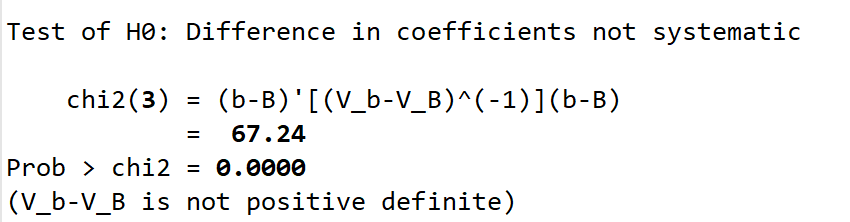
\includegraphics{Hausman.png}
\end{figure}

Hausman test output yields a chi-square statistic of 61.64 (with p-value$ = 0.0000$).

The null hypothesis is strongly rejected, indicating that the RE estimator is inconsistent and that the FE estimator is preferred.
\end{autosolution}

\begin{autosolution}
    \

    Let$\theta = \beta_1 + \beta_2$. Under the null hypothesis, we have
    \[
    H_0: \theta = 1.
    \]
    An estimator for $\theta$ is
    \[
    \hat{\theta} = \hat{\beta}_1 + \hat{\beta}_2.
    \]
    Suppose the estimated coefficients $\hat{\beta}_1$ and $\hat{\beta}_2$ have the following variance-covariance matrix:
    \[
    V = \begin{pmatrix}
    \operatorname{Var}(\hat{\beta}_1) & \operatorname{Cov}(\hat{\beta}_1, \hat{\beta}_2) \\
    \operatorname{Cov}(\hat{\beta}_1, \hat{\beta}_2) & \operatorname{Var}(\hat{\beta}_2)
    \end{pmatrix}.
    \]
    Because $\hat{\theta}$ is a sum of $\hat{\beta}_1$ and $\hat{\beta}_2$, by the properties of variance we have:
    \[
    \operatorname{Var}(\hat{\theta}) = \operatorname{Var}(\hat{\beta}_1 + \hat{\beta}_2) = \operatorname{Var}(\hat{\beta}_1) + \operatorname{Var}(\hat{\beta}_2) + 2\,\operatorname{Cov}(\hat{\beta}_1, \hat{\beta}_2).
    \]
    Under $\mathcal{H}_0$, the deviation of $\hat{\theta}$ from its hypothesized value is:
    \[
    \hat{\theta} - 1 = \hat{\beta}_1 + \hat{\beta}_2 - 1.
    \]
    Since, by the Central Limit Theorem, $\hat{\theta}$ is approximately normally distributed in large samples, we can standardize the difference:
    \[
    Z = \frac{\hat{\theta} - 1}{\sqrt{\operatorname{Var}(\hat{\theta})}}.
    \]
    Under $H_0$, $Z$ is asymptotically standard normal. Squaring this $Z$ statistic gives a chi-square statistic with 1 degree of freedom:
    \[
    \chi^2 = \frac{(\hat{\beta}_1 + \hat{\beta}_2 - 1)^2}{\operatorname{Var}(\hat{\beta}_1) + \operatorname{Var}(\hat{\beta}_2) + 2\,\operatorname{Cov}(\hat{\beta}_1, \hat{\beta}_2)}.
    \]
    This test statistic is compared to the $\chi^2_1$ distribution.
    \begin{itemize}
        \item If $\chi^2$ is large (and the corresponding p-value is small), we reject $H_0$ and conclude that the sum of $\beta_1$ and $\beta_2$ is statistically different from 1.  
        \item If $\chi^2$ is not large (and the p-value is large), we do not reject $H_0$ and there is no evidence against constant returns to scale.
    \end{itemize}

    At the conventional 5\% level, the p-value (0.0000) is much smaller than 0.05, meaning we reject $\mathcal{H}_0$.
    \begin{figure}[htbp!]
        \centering
        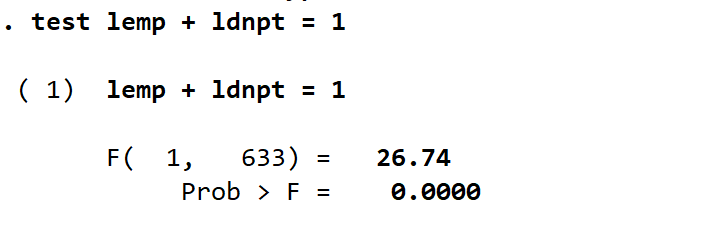
\includegraphics[width=0.5\textwidth]{F_test.png}
    \end{figure}
\end{autosolution}

\end{document}

